\documentclass{article}
\usepackage[utf8]{inputenc}
\usepackage[left=3cm, right=3cm, top=2cm]{geometry}
\title{Modal Analysis}
\author{Silvin Willemsen}
\date{February 2021}
\usepackage{natbib}
\usepackage{graphicx}
\usepackage{appendix}
\usepackage{amsmath}
\usepackage{amsfonts}
\usepackage{amssymb}
\usepackage{extarrows}
\usepackage{xcolor} 
\def\SWcomment[#1]{\textcolor{blue}{#1}}

% \usepackage{natbib}

\def\mystrut{\rule[-.2\baselineskip]{0pt}{\baselineskip}}

\def\u{\mathbf{u}}
\def\w{\mathbf{w}}
\def\I{\mathbf{I}}
\def\A{\mathbf{A}}
\def\B{\mathbf{B}}
\def\C{\mathbf{C}}
\def\Q{\mathbf{Q}}

\def\Dxx{\mathbf{D}_{xx}}
\def\Dxxxx{\mathbf{D}_{xxxx}}

\begin{document}

\maketitle

\section{Introduction}
In this document I will go through the matrix form of some schemes and how these can be analyses to obtain the modes of these systems. I will follow Section 6.2.8 of \cite{Bilbao2009}.

% \begin{figure}[h!]
% \centering
% \includegraphics[scale=1.7]{universe}
% \caption{The Universe}
% \label{fig:universe}
% \end{figure}
\section{Preamble}
\subsection{Identities}
Sin identity:
\begin{equation}\label{eq:sinIdentity}
    \sin(x) = \frac{e^{jx} - e^{-jx}}{2j}\quad \Longrightarrow \quad \sin^2(x) = \frac{e^{j2x} - 2e^{jx-jx}+ e^{-j2x}}{-4} = \frac{e^{j2x} + e^{-j2x}}{-4} + \frac{1}{2}.
\end{equation}
Cos identity:
\begin{equation}\label{eq:cosIdentity}
    \cos(x) = \frac{e^{jx} + e^{-jx}}{2}\quad \Longrightarrow \quad \cos^2(x) = \frac{e^{j2x} + 2e^{jx-jx}+ e^{-j2x}}{4} = \frac{e^{j2x} + e^{-j2x}}{4} + \frac{1}{2}.
\end{equation}

% From this we can derive the useful identity for $\sin^4(x)$:

% \begin{align}
%     \sin^4(x) = (\sin^2(x))^2 &= \Bigg(\frac{e^{j2x} + e^{-j2x}}{-4} + \frac{1}{2}\Bigg)^2\nonumber\\
%     &=\Bigg(\frac{e^{j2x} + e^{-j2x}}{-4}\Bigg)^2 + \frac{e^{j2x} + e^{-j2x}}{-4} + \frac{1}{4}\nonumber\\
%     &=\frac{e^{j4x} + e^{-j4x}}{16} + \frac{1}{8} + \underbrace{\frac{e^{j2x} + e^{-j2x}}{-4}}_\text{$\sin^2(x)- \frac{1}{2}$} + \frac{1}{4}\nonumber\\
%     &= -\frac{1}{4}\Bigg(\frac{e^{j4x} + e^{-j4x}}{-4} + \frac{1}{2}\Bigg) + \frac{2}{8} + \sin^2(x) - \frac{1}{2} + \frac{1}{4}\nonumber\\
%     &= -\frac{1}{4}\sin^2(2x) + \sin^2(x) \label{eq:sin4}
% \end{align}
% \subsection{Frequency domain analysis}
% See section 5.2.6 of \cite{Bilbao2009}:
% \begin{equation}
%     u_l^n = z^n e^{jl\beta h}
% \end{equation}
% where $\beta$ is a real wavenumber. Important to remember is that without a shift in space (fx. $l+1$) or time (fx. $n-1$) $l = 0$ or $n=0$ respectively:
% \begin{subequations} \label{eq:identitiesZ}
%     \begin{align}
%         u_l^n &= z^0 e^{j0\beta h} = 1\\
%         u_{l+1}^n &= z^0 e^{j1\beta h} = e^{j\beta h}\\
%         u_{l-1}^n &= z^0 e^{j(-1)\beta h} = e^{-j\beta h}\\
%         u_{l+2}^n &= z^0 e^{j2\beta h} = e^{j\beta h}\\
%         u_{l-2}^n &= z^0 e^{j(-2)\beta h}= e^{-j2\beta h}\\
%         u_l^{n+1}&= z^1 e^{j0\beta h} = z\\
%         u_l^{n-1}&= z^{-1} e^{j0\beta h} = z^{-1}
%     \end{align}
% \end{subequations}
\subsection{Operators in Matrix Form}
Finite-difference operators, such as $\delta_{x+}$,  $\delta_{x-}$ and $\delta_{x\cdot}$ can be written in matrix form:
\begin{gather*}
    \mathbf{D}_{x+} = \frac{1}{h}\begin{bmatrix}
        \ddots &\ddots & & & \mathbf{0}&\\
         & -1 & 1 & & & \\
        & & -1 & 1 & & \\
        & & & -1 & 1 & \\
        & & & & -1 & \ddots\\
        &\mathbf{0} & & & & \ddots \\
    \end{bmatrix}
    \qquad
    \mathbf{D}_{x-} = \frac{1}{h}\begin{bmatrix}
        \ddots & & & & \mathbf{0}&\\
        \ddots & 1 & & & & \\
        & -1 & 1 & & & \\
        & & -1 & 1 & & \\
        & & & -1 & 1 & \\
        &\mathbf{0} & & & \ddots & \ddots \\
    \end{bmatrix}\\
    \\
    \mathbf{D}_{x\cdot} = \frac{1}{2h}\begin{bmatrix}
        \ddots &\ddots & & & \mathbf{0}&\\
        \ddots & 0 & 1 & & & \\
        & -1 & 0 & 1 & & \\
        & & -1 & 0 & 1 & \\
        & & & -1 & 0 & \ddots \\
        &\mathbf{0} & & & \ddots & \ddots \\
    \end{bmatrix}\\
\end{gather*}
The matrices $\mathbf{D}_{x+}$ and $\mathbf{D}_{x-}$ can be multiplied to get $\Dxx$:
\begin{equation}
    \Dxx = \mathbf{D}_{x+}\mathbf{D}_{x-} = \frac{1}{h^2}\begin{bmatrix}
        \ddots &\ddots & & & \mathbf{0}&\\
        \ddots & -2 & 1 & & & \\
        & 1 & -2 & 1 & & \\
        & & 1 & -2 & 1 & \\
        & & & 1 & -2 & \ddots \\
        &\mathbf{0} & & & \ddots & \ddots \\
    \end{bmatrix}
\end{equation}
and two $\Dxx$'s to get
\begin{equation}
    \Dxx\Dxx = \mathbf{D}_{xxxx} = \frac{1}{h^4}\begin{bmatrix}
        5& -4 & 1 & & & \mathbf{0}& \\
        -4 & 6 &\ddots &\ddots & & & \\
        1& \ddots & \ddots & -4 & 1 & & \\
        & \ddots& -4 & 6 & -4 & \ddots& \\
        & & 1 & -4 & \ddots & \ddots &1 \\
        & & & \ddots & \ddots & 6 & -4 \\
        & \mathbf{0} & & & 1& -4 & 5 \\
    \end{bmatrix}
\end{equation}
which is used for a stiff string with a simply supported boundary condition.

Averaging operators $\mu_{x+}$, $\mu_{x-}$ and $\mu{x\cdot}$ are defined in a similar way:
\begin{gather*}
    \mathbf{M}_{x+} = \frac{1}{2}\begin{bmatrix}
        \ddots &\ddots & & & \mathbf{0}&\\
         & 1 & 1 & & & \\
        & & 1 & 1 & & \\
        & & & 1 & 1 & \\
        & & & & 1 & \ddots\\
        &\mathbf{0} & & & & \ddots \\
    \end{bmatrix}
    \qquad
    \mathbf{M}_{x-} = \frac{1}{2}\begin{bmatrix}
        \ddots & & & & \mathbf{0}&\\
        \ddots & 1 & & & & \\
        & 1 & 1 & & & \\
        & & 1 & 1 & & \\
        & & & 1 & 1 & \\
        &\mathbf{0} & & & \ddots & \ddots \\
    \end{bmatrix}\\
    \\
    \mathbf{M}_{x\cdot} = \frac{1}{2}\begin{bmatrix}
        \ddots &\ddots & & & \mathbf{0}&\\
        \ddots & 0 & 1 & & & \\
        & 1 & 0 & 1 & & \\
        & & 1 & 0 & 1 & \\
        & & & 1 & 0 & \ddots \\
        &\mathbf{0} & & & \ddots & \ddots \\
    \end{bmatrix}\\
\end{gather*}
Note the multiplication by $1/2$ rather than $1/h$ (or $1/2h$) for all operators.


Only spatial operators are written in this matrix form and then applied to state vectors at different time steps ($n+1$, $n$ and $n-1$), examples of which can be found below.

\section{1D Wave Equation}
This section will show how to obtain the modes for an FDS implementing the 1D wave equation as done in Section . We start with Eq. (6.34)
\begin{equation}
    \delta_{tt}u = \gamma^2\delta_{xx}u,
\end{equation}
which can be written in matrix form as
\begin{equation}\label{eq:matrixForm1D}
    \frac{1}{k^2}\left(\u^{n+1}-2\u^n+\u^{n-1}\right) = \gamma^2 \Dxx\u
\end{equation}
Following \cite{Bilbao2009} we assume a solution of the form $\u = \boldsymbol{\phi}z^n$. Substituting this into Eq. \eqref{eq:matrixForm1D} yields the characteristic equation
\begin{equation}
    (z - 2 + z^{-1})\boldsymbol{\phi} = \gamma^2k^2\Dxx \boldsymbol{\phi}.
\end{equation}
This is an eigenvalue problem where the $p$'th solution is defined as 
\begin{gather}
    z_p-2+z_p^{-1} = \gamma^2k^2\text{eig}_p(\Dxx)\nonumber\\
    z_p+(-2-\gamma^2k^2\text{eig}_p(\Dxx))+z_p^{-1}=0
\end{gather}
where $\text{eig}_p(\cdot)$ denoting the $p$th eigenvalue of `$\cdot$'. \SWcomment[If the CFL condition for the scheme is satisfied, the roots will lie on the unit circle.] Furthermore we can substitute a test solution $z_p=e^{j\omega_pk}$ solve for the eigenfrequencies:
\begin{align*}
    e^{j\omega_pk}+e^{-j\omega_pk}-2-\gamma^2k^2\text{eig}_p(\Dxx)&=0\\
    \frac{e^{j\omega_pk}+e^{-j\omega_pk}}{-4}+\frac{1}{2}+\frac{\gamma^2k^2}{4}\text{eig}_p(\Dxx)&=0
\end{align*}
Then using Eq. \eqref{eq:sinIdentity} we get
\begin{align}
    \sin^2(\omega_pk/2)+\gamma^2k^2\text{eig}_p(\Dxx)&=0\nonumber\\
    \sin(\omega_pk/2)&=\gamma k\sqrt{-\text{eig}_p(\Dxx)}\nonumber\\
    \omega_p &= \frac{2}{k}\sin^{-1}\left(\gamma k\sqrt{-\text{eig}_p(\Dxx)}\right)
\end{align}
which is Eq. (6.53) in \cite{Bilbao2009}.

\section{Implicit Ideal Bar}
Just for clarity, a derivation of the equation calculating frequencies for the implicit ideal bar found in \cite[Section 7.1.5, p. 174]{Bilbao2009}. Starting from Eq. (7.17)
\begin{equation}
    (\theta + (1-\theta)\mu_{x\cdot})\delta_{tt}u = -\kappa^2\delta_{xxxx}u
\end{equation}
and writing this in matrix form gives

\begin{gather*}
    \underbrace{(\theta \I + (1-\theta)\mathbf{M}_{x\cdot})}_{\A}\frac{1}{k^2}(\u^{n+1} - 2\u^n + \u^{n-1}) = -\kappa^2\mathbf{D}_{xxxx}\u^n\\
    \begin{aligned}
    \A\u^{n+1} &= \underbrace{(2\A-\kappa^2k^2\mathbf{D}_{xxxx})}_{\B}\u^n - \A\u^{n-1}\\
    \u^{n+1} &= \A^{-1}\B\u^n - \u^{n-1}
    \end{aligned}
\end{gather*}
We can then again assume $\u = \boldsymbol{\phi}z^n$ and substitute to get characteristic equation
\begin{equation}
    (z + z^{-1})\boldsymbol{\phi} = (\A^{-1}\B)\boldsymbol{\phi}
\end{equation}
with solutions
\begin{align*}
    z_p + z_p^{-1} &= \text{eig}_p(\A^{-1}\B)\\
 z_p -\text{eig}_p(\A^{-1}\B) + z_p^{-1} &= 0.
\end{align*}
Substituting $z_p = e^{j\omega_pk}$ yields
\begin{align*}
    e^{j\omega_pk}+e^{-j\omega_pk} - \text{eig}_p(\A^{-1}\B) = 0\\
    \frac{e^{j\omega_pk}+e^{-j\omega_pk}}{2} - \frac{1}{2}\text{eig}_p(\A^{-1}\B) = 0
\end{align*}
and using Eq. \eqref{eq:cosIdentity}
\begin{align}
    \cos(\omega_pk) = \frac{1}{2}\text{eig}_p(\A^{-1}\B)\nonumber\\
    \omega_p =\frac{1}{k}\cos^{-1}\left(\frac{1}{2}\text{eig}_p(\A^{-1}\B)\right)\nonumber\\
    f_p =\frac{1}{2\pi k}\cos^{-1}\left(\frac{1}{2}\text{eig}_p(\A^{-1}\B)\right)
\end{align}
which is the equation found in \cite[p. 174]{Bilbao2009}.

\section{Rewriting to One-Step Form}
For more complicated systems, where the coefficients of $z$ and $z^{-1}$ are not identical for example, it is useful to rewrite the update in one-step form. Any scheme of the form
\begin{equation}
    \A\u^{n+1}=\B\u^n + \C\u^{n-1},
\end{equation}
can be rewritten to
\begin{equation}\label{eq:oneStepForm}
    \underbrace{\begin{bmatrix}
        \u^{n+1}\\
        \u^n
    \end{bmatrix}}_{\w^{n+1}} = 
    \underbrace{\begin{bmatrix}
        \A^{-1}\B & \A^{-1}\C\\
        \I & \mathbf{0}
    \end{bmatrix}}_{\Q}
    \underbrace{\begin{bmatrix}
        \u^n\\
        \u^{n-1}
    \end{bmatrix}}_{\w^n}
\end{equation}
which relates the unknown state of the system to the known state through matrix $\Q$ which encompases the scheme. The sizes of the identity matrix $\I$ and zero matrix $\mathbf{0}$ are the same size as $\A, \B$ and $\C$ and are essentially used to make the matrix square and allow for eigenvalue calculation.

Again we can assume solutions of the form $\w = z^n\boldsymbol{\phi}$ and get
\begin{equation}
    z\boldsymbol{\phi} = \Q\boldsymbol{\phi} 
\end{equation}
and solved for the $p$th eigenvalue as
\begin{equation}
    z_p = \text{eig}_p(\Q)
\end{equation}
As the scheme could exhibit damping, the test solution need to include this and will be $z_p = e^{s_pk}$ with complex frequency $s_p= j\omega_p + \sigma_p$ and damping of the $p$th eigenfrequency $\sigma_p$.

\begin{align}
    e^{s_pk} &= \text{eig}_p(\Q)\nonumber\\
    s_p &= \frac{1}{k}\ln \left(\text{eig}_p(\Q)\right)\label{eq:sp}
\end{align}
Solutions for the frequency and damping for the $p$th eigenvalue can then be obtained through
\begin{equation}
    \omega_p = \mathfrak{I}(s_p) \quad \text{and} \quad \sigma_p = \mathfrak{R}(s_p)
\end{equation}
where $\mathfrak{I}$ and $\mathfrak{R}$ denote the ``imaginary" and ``real part of" respectively. 

As the elements of $\Q$ are real-valued, the solutions $s_p$ in Eq. \eqref{eq:sp} come in complex conjugates. For analysis, only the $\mathfrak{I}(s_p)\geq 0$ should be considered as these correspond to non-negative frequencies.

\subsection{Damped stiff string}
To test the one-step from, we can take the damped stiff string as an example. There are two versions available:
\begin{subequations}
    \begin{align}
        \delta_{tt}u &= c^2\delta_{xx}u - \kappa^2\delta_{xxxx}u - 2\sigma_0\delta_{t\cdot}u + 2\sigma_1\delta_{t-}\delta_{xx}u,\label{eq:dampedStiffStringExp}\\
        \delta_{tt}u &= c^2\delta_{xx}u - \kappa^2\delta_{xxxx}u - 2\sigma_0\delta_{t\cdot}u + 2\sigma_1\delta_{t\cdot}\delta_{xx}u\label{eq:dampedStiffStringImp},
    \end{align}
\end{subequations}
as Eq. (7.30) in \cite{Bilbao2009}. The first is explicit, and the second is implicit due to the centered difference operator in the frequency dependent damping term. This has the added advantage that $\sigma_1$ does not have to be included in the definition for the stability condition. Writing Eq. \eqref{eq:dampedStiffStringExp} in matrix form yields
\begin{equation}
    \begin{aligned}
        (1+\sigma_0k)\I \u^{n+1} =& \left(2\I + c^2k^2\Dxx -\kappa^2k^2\Dxxxx + 2\sigma_1k\Dxx\right)\u^n\\
    &- \big((1-\sigma_0k)\I+2\sigma_1k\Dxx\big)\u^{n-1}.
    \end{aligned}
\end{equation}
Relating this to the one-step form in Eq. \eqref{eq:oneStepForm} we get the following matrices
\begin{equation}
    \begin{gathered}
        \A = (1+\sigma_0k)\I, \quad \B =2\I + c^2k^2\Dxx -\kappa^2k^2\Dxxxx + 2\sigma_1k\Dxx \\
        \quad \text{and} \quad \C = - \big((1-\sigma_0k)\I+2\sigma_1k\Dxx\big).
    \end{gathered}
\end{equation}
The implicit scheme in Eq. \eqref{eq:dampedStiffStringImp} yields the following matrices
\begin{equation}
    \begin{gathered}
        \A = (1+\sigma_0k)\I - 2\sigma_1k\Dxx, \quad \B =2\I + c^2k^2\Dxx -\kappa^2k^2\Dxxxx \\
        \quad \text{and} \quad \C = - \big((1-\sigma_0k)\I+2\sigma_1k\Dxx\big).
    \end{gathered}
\end{equation}
These can then be compared and plotted against each other, see Figure \ref{fig:expImpComp}. The following values are used: $c = 1470$, $\kappa = 0$ (for clarity in the figure), $\sigma_0 = 1$, $\sigma_1 = 1$. It can be observed that, due to the backwards-time implementation of the frequency dependent damping term, the stability condition is stricter and allows for fewer grid points and thus fewer modes. Furthermore, this causes a decrease in bandwidth and inharmonicity in the higher frequency ranges.

\begin{figure}
    \centering
    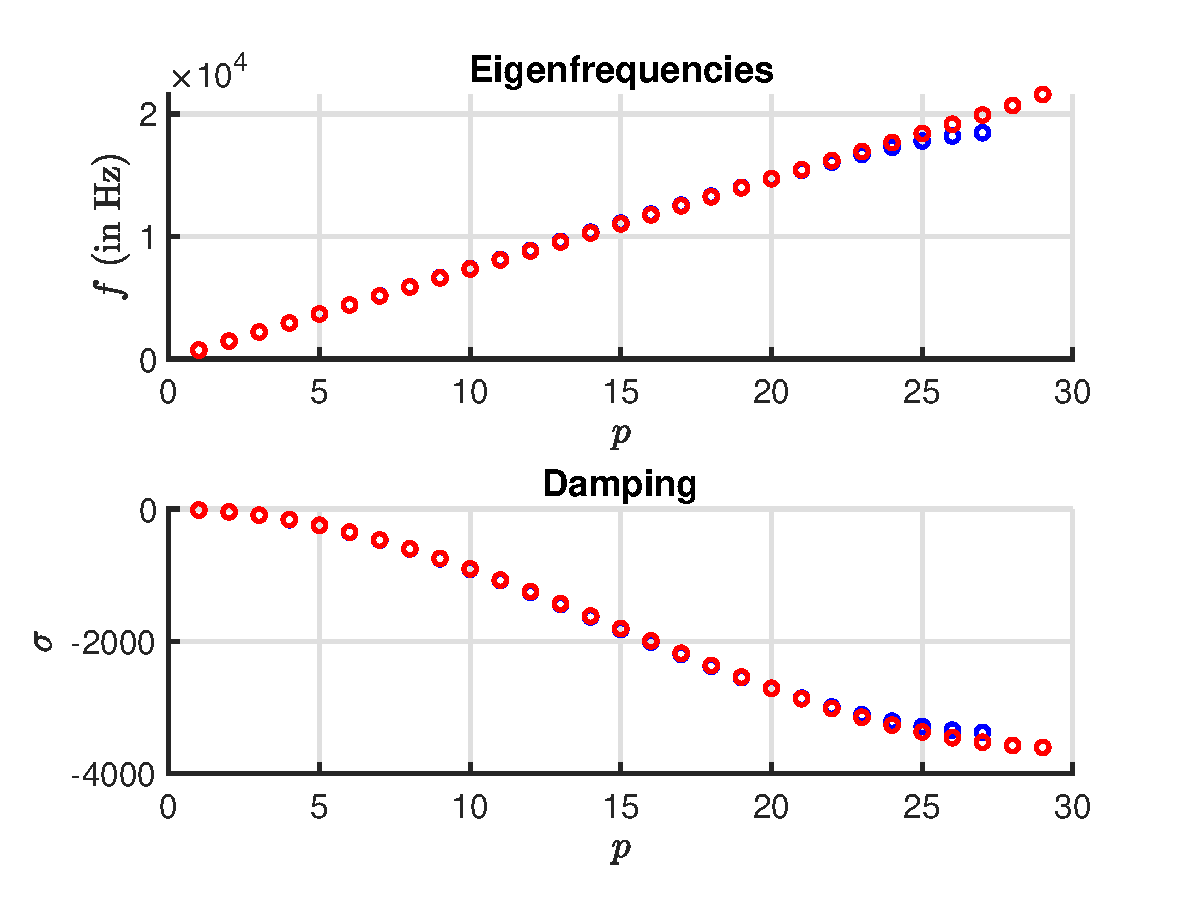
\includegraphics[width = 0.8\textwidth]{expImpComp.eps}
    \caption{Comparison between modal analysis of the damped stiff string with explicit and implicit damping. The results for the analysis of the explicit scheme are shown in blue, the implicit in red.}
    \label{fig:expImpComp}
\end{figure}
\bibliographystyle{plain}
\bibliography{references}
\end{document}
